\section{Action-Level Transfer}
Action-level differences stem from how commands translate to real actuators. Simulators often assume ideal, synchronous action execution, whereas real robots have continuous-time dynamics, delays, saturations, and noise. Key challenges include actuator latency, unmodeled torque limits, and quantization (e.g. servos that only accept discrete commands).

A straightforward remedy is to \emph{model the actuator dynamics and noise} in simulation. For instance, injecting random motor noise, friction variation, and delays during training produces policies that are robust to these effects. OpenAI’s Dactyl system (dexterous hand manipulation) used extensive randomization of physical properties (finger friction, motor strength, mass of objects) so that the learned policy could tolerate real actuator uncertainties\cite{Akkaya2019}. In legged locomotion, Tan et al.\ randomized actuator response times and motor parameters, which improved real-world stability\cite{Tan2018}. This form of domain randomization on the action channel hedges against mismatch by exposing the policy to a range of possible actuator behaviors.

Beyond randomization, more principled methods attempt to \emph{transform actions} between domains. \emph{Grounded Action Transformation} (GAT) learns a mapping that “grounds” simulator actions to mimic real-world effects\cite{Hanna2017}. Essentially, one learns a function $g(a)$ such that executing $a$ in sim has the same outcome as $g(a)$ in real, or vice versa. Variants like SGAT (stochastic GAT) and RGAT (reinforced GAT) extend this idea to handle stochasticity or use RL to learn the transformation\cite{Desai2020,Karnan2020}. These methods explicitly adjust the transition function of the simulator to better match the real robot’s response. For example, if a real robot joint moves slower than the simulator model, GAT would scale down the sim commands so that actions are comparable. \textbf{Figure~\ref{fig:gat_mechanism}} illustrates this principle: a forward model predicts the real-world outcome, which is then inverted through the simulation model to generate a grounded action. In practice, grounded actions require some real data for calibration, but they can significantly reduce the sim-real control mismatch.


\begin{figure}[H]
    \centering
    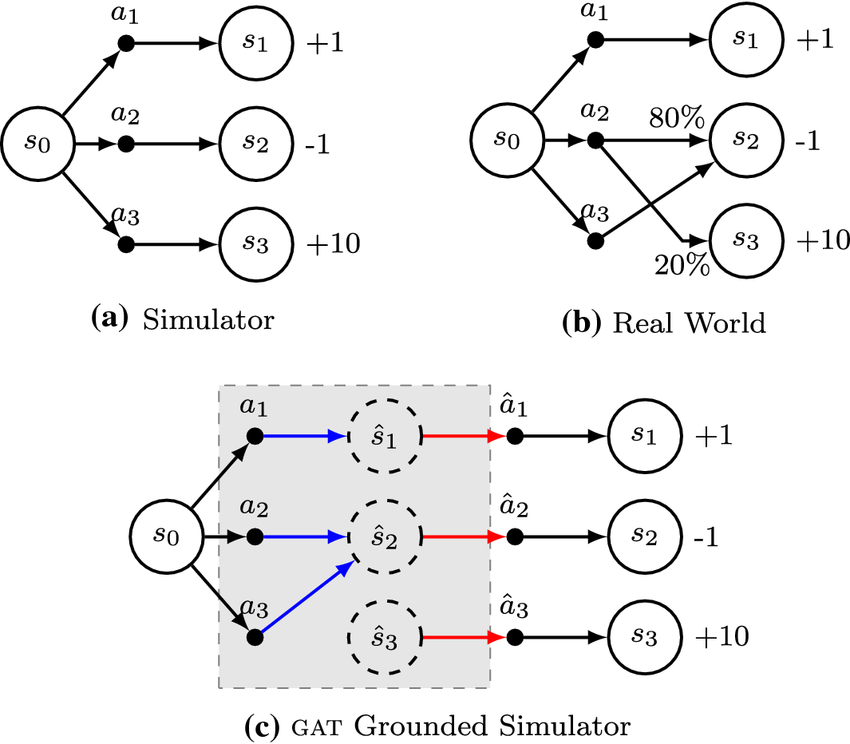
\includegraphics[width=0.95\linewidth]{figures/figGATMechanism.png}
    \caption{Illustration of the Grounded Action Transformation (GAT) mechanism: A forward model $f_{real}$ predicts the next real-world state, which is then mapped back into the simulator action space via the inverse simulation model $f_{sim}^{-1}$. This transformation aims to produce simulator actions that better match real-world effects. (\emph{Source:} Hanna et al., 2021)}
    \label{fig:gat_mechanism}
\end{figure}

Another complementary technique is \textit{robust policy design}, which trains agents to tolerate uncertainty. This includes adversarial training with perturbed actions or robust control frameworks with formal guarantees. Policies trained with adversarial noise tend to ignore small deviations in command execution, improving resilience to mismatches.

In summary, action-level transfer blends randomized modeling and explicit calibration. Randomization (as in Fig.~\ref{fig:adr_pipeline}(B)) can cover many uncertainties but may not capture systematic biases (e.g.\ consistent actuator lag). Grounded action techniques and system identification fill this gap by learning the actual mapping, at the cost of requiring real observations. We encourage combining both: randomize broadly, then fine-tune or adapt the action model with real data for best performance.

\paragraph{Evaluation.} Injecting actuator noise and delays during training improves robustness, as shown in legged locomotion by Tan et al.~\cite{Tan2018}. However, this approach may not fully capture systematic real-world effects such as persistent latency or actuator limits. Grounded Action Transformation (GAT) and its variants~\cite{Hanna2017, Desai2020} offer precise domain alignment, but depend on real-world calibration and are often task-specific. In practice, combining randomized actuation with post-hoc transformation yields better sim-to-real transfer in continuous control settings. Quantitative results from OpenAI's Dactyl system show that randomized actuator properties (e.g., motor noise, friction) enabled the real-world hand to perform more than 13 consecutive object rotations, compared to complete failure without such augmentation \cite{Akkaya2019}. Similarly, grounded action transformations improved humanoid robot walking speed by up to 43\% compared to hand-designed baselines \cite{Hanna2017}.